\documentclass[11pt]{article}
\usepackage[margin=1in]{geometry}
\usepackage[utf8]{inputenc}
\usepackage[T1]{fontenc}
\usepackage{amsmath,amssymb,amsthm,mathtools,braket,enumitem,graphicx,tikz,hyperref}
\usetikzlibrary{arrows.meta,calc,positioning,shapes.geometric,decorations.pathmorphing}
\hypersetup{colorlinks=true, linkcolor=blue!50!black, urlcolor=blue!50!black}

\newcommand{\vecb}[1]{\vec{#1}}
\newcommand{\hbf}[1]{\hat{#1}}
\newcommand{\mubohr}{\mu_B}

\title{Quantum Optics --- Lecture 2\\ \large Two-level atomic systems: Stern--Gerlach and spin $\tfrac12$}
\author{Transcribed from handwritten notes (Note Sep 15, 2026, pp.\,3--7)}
\date{}

\begin{document}
\maketitle

\section*{Two level atomic systems}

\subsection*{Stern--Gerlach + Spin $\tfrac12$}

\[
  \braket{\vecb{\mu}} = -g\,\mubohr \Braket{\frac{\vecb{J}}{\hbar}}
\]

\begin{center}
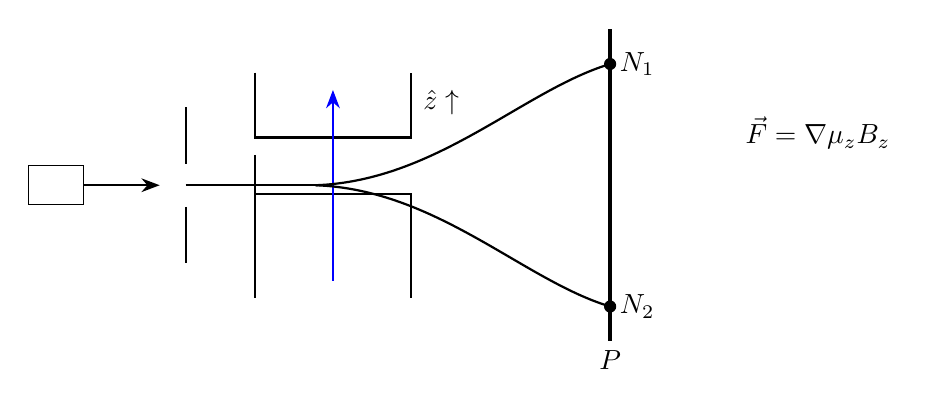
\begin{tikzpicture}[>=Stealth, scale=1.1]
  % oven / incoming beam
  \node[draw, minimum width=0.7cm, minimum height=0.5cm] (oven) at (-3.2,0) {};
  \draw[->, thick] (oven.east) -- (-2.0,0);
  % collimating slit
  \draw[thick] (-1.7,0.9) -- (-1.7,0.25);
  \draw[thick] (-1.7,-0.25) -- (-1.7,-0.9);
  % magnet poles (N on top, S below), inhomogeneous field along z
  \draw[thick] (-0.9,1.3) -- (-0.9,0.55) -- (0.9,0.55) -- (0.9,1.3);
  \draw[thick] (-0.9,0.35) -- (-0.9,-0.1) -- (0.9,-0.1) -- (0.9,-1.3);
  \draw[thick] (-0.9,-0.1) -- (-0.9,-1.3);
  \draw[->, blue, thick] (0,-1.1) -- (0,1.1);
  \node at (1.25,0.95) {$\hbf{z}\uparrow$};
  % beam and split
  \draw[thick] (-1.7,0) -- (-0.2,0);
  \draw[thick] (-0.2,0) .. controls (1.2,0.05) and (2.2,1.1) .. (3.2,1.4);
  \draw[thick] (-0.2,0) .. controls (1.2,-0.05) and (2.2,-1.1) .. (3.2,-1.4);
  % detection plate
  \draw[very thick] (3.2,1.8) -- (3.2,-1.8);
  \fill (3.2,1.4) circle (2pt) node[right] {$N_1$};
  \fill (3.2,-1.4) circle (2pt) node[right] {$N_2$};
  \node[below] at (3.2,-1.8) {$P$};
  % force
  \node at (5.6,0.6) {$\vecb{F} = \nabla \mu_z B_z$};
\end{tikzpicture}
\end{center}

Interaction energy of the magnetic moment with the magnetic field is just $-\vecb{\mu}\cdot\vecb{B}$.
\[
  F_z = \frac{\partial}{\partial z}\bigl(\vecb{\mu}\cdot\vecb{B}\bigr) \simeq \mu_z \frac{\partial B_z}{\partial z}
\]

\begin{itemize}
  \item If $\mu_z > 0$ ($S_z < 0$) the atom experiences an upward force.
  \item If $\mu_z < 0$ ($S_z > 0$) the atom experiences a downward force.
  \item The atoms in the furnace are randomly oriented. So classically we would expect values between $|\mu|$ and $-|\mu|$; this would lead to a spread in the values, unlike the only two spots being observed.
\end{itemize}

\begin{itemize}[label=$\Rightarrow$]
  \item Later this was realized to be spin.
  \item We also see the weird measurement effects with multiple Stern--Gerlach experiments.
\end{itemize}

\[
  \vecb{E} = E_0\,\hbf{x}\cos(kz - \omega t)
\]
Likewise we may consider $y$-polarized light, also propagating in the $z$-direction
\[
  \vecb{E} = E_0\,\hbf{y}\cos(kz - \omega t)
\]

Then we have that
\begin{center}
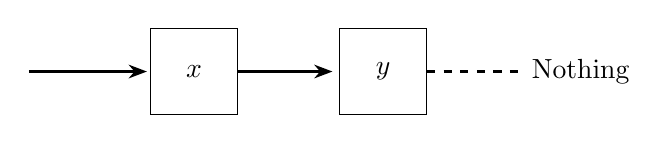
\begin{tikzpicture}[>=Stealth, box/.style={draw, minimum width=1.1cm, minimum height=1.1cm}]
  \draw[->, thick] (-1.5,0) -- (0,0);
  \node[box] (x) at (0.6,0) {$x$};
  \draw[->, thick] (x.east) -- ++(1.2,0);
  \node[box] (y) at (3.0,0) {$y$};
  \draw[dashed, thick] (y.east) -- ++(1.2,0) node[right] {Nothing};
\end{tikzpicture}
\end{center}
but
\begin{center}
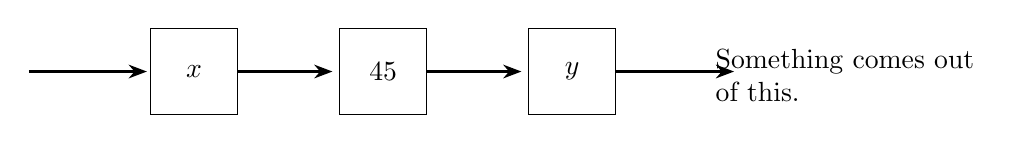
\begin{tikzpicture}[>=Stealth, box/.style={draw, minimum width=1.1cm, minimum height=1.1cm}]
  \draw[->, thick] (-1.5,0) -- (0,0);
  \node[box] (x) at (0.6,0) {$x$};
  \draw[->, thick] (x.east) -- ++(1.2,0);
  \node[box] (m) at (3.0,0) {$45$};
  \draw[->, thick] (m.east) -- ++(1.2,0);
  \node[box] (y) at (5.4,0) {$y$};
  \draw[->, thick] (y.east) -- ++(1.5,0);
  \node[align=left, anchor=west] at (7.1,-0.05) {Something comes out\\ of this.};
\end{tikzpicture}
\end{center}

\subsection*{Constructing spin operators from sequential SG experiments}

We know we can write
\[
  S_z = \frac{\hbar}{2}\Bigl[\ket{+}\bra{+} - \ket{-}\bra{-}\Bigr]
\]

Classically a current loop has the magnetic moment
\begin{align*}
  \mu = \frac{IA}{c} &= \frac{qA}{Tc} = \frac{qvA}{2\pi r\, c} = \frac{qv\,\pi r^2}{2\pi r\, c} \\
  &= \frac{qv}{2c}\, r = \frac{q}{2mc}\, m v r = \frac{q}{2mc}\, L
\end{align*}
so
\[
  \mu = \frac{q}{2mc}\, L .
\]
For spin $\displaystyle \mu = g\,\frac{q}{2mc}\, S$; $g = 1 \Rightarrow$ classical orbital value. Dirac says $g = 2$:
\[
  \mu = \frac{q}{mc}\, S .
\]
\[
  |S_z| = \frac{m_e c}{e}\,|\mu_z|, \qquad \mu_z = \frac{e\hbar}{2 m_e c}\ \text{(exp.)} \quad \Rightarrow\quad S_z = \frac{\hbar}{2}.
\]

We have that
\[
  \boxed{\, S_z = \frac{\hbar}{2}\Bigl[\ket{+}\bra{+} - \ket{-}\bra{-}\Bigr] \,}
\]

\paragraph{Obs:} the $S_x+$ beam splits 50/50 in SG$\hbf{z}$, so we require that
\[
  \bigl|\braket{+|S_x;+}\bigr|^2 = \bigl|\braket{-|S_x;-}\bigr|^2 = \frac12
\]
but it also must be the case that
\[
  \ket{S_x;+} = c_1\ket{+} + c_2\ket{-} ,
\]
thus combining the two and taking into account an unphysical phase we have that
\[
  \ket{S_x;+} = \frac{1}{\sqrt2}\ket{+} + \frac{e^{i\delta_1}}{\sqrt2}\ket{-} .
\]
Then since $\ket{S_x;-}$ is necessarily orthogonal to $\ket{S_x;+}$ we have that
\[
  \ket{S_x;-} = \frac{1}{\sqrt2}\ket{+} - \frac{e^{i\delta_1}}{\sqrt2}\ket{-} .
\]

\paragraph{Obs:} $S_y+$ also splits in SG$x$, so
\begin{align*}
  \braket{S_y;+|S_x;+} &= \frac12\bigl(1 + e^{i(\delta_1-\delta_2)}\bigr) \\
  \bigl|\braket{S_y;+|S_x;-}\bigr|^2 &= \frac14\bigl|1 + e^{i(\delta_1-\delta_2)}\bigr|^2
    = \frac12\bigl(1 + \cos(\delta_1-\delta_2)\bigr) = \frac12 \\
  &\iff \cos(\delta_1-\delta_2) = 0 \iff \delta_2 - \delta_1 = \pm\frac{\pi}{2}
\end{align*}
Let $\delta = \dfrac{\pi}{2}$, so
\[
  \ket{S_x;\pm} = \frac{1}{\sqrt2}\bigl(\ket{+} \pm \ket{-}\bigr)
  \qquad\text{and}\qquad
  \ket{S_y;\pm} = \frac{1}{\sqrt2}\bigl(\ket{+} \pm i\ket{-}\bigr) .
\]
So
\begin{align*}
  S_x &= \frac{\hbar}{2}\Bigl(\ket{S_x;+}\bra{S_x;+} - \ket{S_x;-}\bra{S_x;-}\Bigr) \\
      &= \frac{\hbar}{2}\Bigl(\ket{+}\bra{-} + \ket{-}\bra{+}\Bigr) \\[4pt]
  S_y &= \frac{\hbar}{2}\Bigl(-i\ket{+}\bra{-} + i\ket{-}\bra{+}\Bigr) .
\end{align*}

\end{document}
